\documentclass[12pt]{article}

\usepackage{amsmath}
\usepackage{amssymb}
\usepackage{geometry}
\usepackage{graphicx}
\usepackage{hyperref}

\geometry{letterpaper,tmargin=1in,bmargin=1in,lmargin=1in,rmargin=1in}

\hypersetup{
colorlinks, linkcolor=blue,
}


\begin{document}

\title{Analog Electronics}
\author{Laboratory exercise 1}
\date{Fall 2016}
\maketitle

\newpage
\section{Abstract}

The purpose of this laboratory exercise is to refresh skills learned from both circuits 1 and 2. Through the use of Multi-Sim and our lab bench equipment we will calculate and graph the cutoff frequency of a low-pass filter.


\section{Theory}
\label{sec:desigan_and_analysis}

Figure \ref{fig:lab1_circuit} shows the circuit that will be constructed during this experimentation. Through the use of the function generator we will be able input an AC voltage at $V_i$. Using the oscilloscope we can measure the output voltage across the capacitor. From that we can derive our amplitude measurements. 

\begin{figure}[!h]
	\centering
	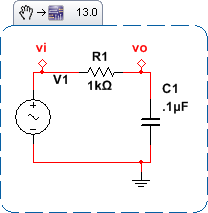
\includegraphics[width=0.4\textwidth]{lab1_circuit.png}
	\caption{A simple low-pass filter}
	\label{fig:lab1_circuit}
\end{figure}
\newpage

\section{Experiment}
\subsection{Experimental setup and procedure}
Using \figurename{1} as our reference for the circuit design we begin the experimentation
\begin{enumerate}
	\item First we construct the circuit ensuring to have all values correct.
	\item By varying the frequency by intervals of 100hz and taking the amplitude at each point, construct a table of all values to model frequency response
\end{enumerate}

\section{Measurements}
\subsection{Measurement Table}

From the data gathered in 3.1.2 we can construct a table.
\begin{table}[h!]
	\centering
	\caption{Measured Voltage at various frequency}
	\label{my-label}
	\begin{tabular}{lllll}

		Frequency & Amplitude & Voltage pk &  &  \\
		500       & 0.7       & 1.4        &  &  \\
		600       & 0.69      & 1.38       &  &  \\
		700       & 0.675     & 1.35       &  &  \\
		800       & 0.665     & 1.33       &  &  \\
		900       & 0.655     & 1.31       &  &  \\
		1000      & 0.65      & 1.3        &  &  \\
		1100      & 0.625     & 1.25       &  &  \\
		1200      & 0.605     & 1.21       &  &  \\
		1300      & 0.59      & 1.18       &  &  \\
		1400      & 0.57      & 1.14       &  &  \\
		1500      & 0.545     & 1.09       &  &  \\
		1600      & 0.52      & 1.04       &  &  \\
		1700      & 0.5       & 1          &  &  \\
		1800      & 0.4915    & 0.983      &  &  \\
		1900      & 0.4725    & 0.945      &  &  \\
		2000      & 0.4575    & 0.915      &  & 
	\end{tabular}
\end{table}
\newpage
\subsection{Graph of Measurements}	

\begin{figure}[h]
	\centering
	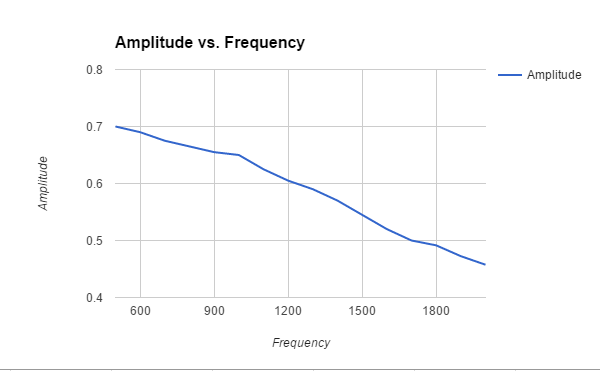
\includegraphics[width=0.8\textwidth]{graph.png}
	\caption{Graph}
	\label{fig:graph}
\end{figure}	

\subsection{Calculating cutoff frequency}

To calculate our cutoff frequency we will use the equation

$$\frac{1}{2\pi RC} = f_c$$

Using our Resistor Value of $1k$ and our Capacitance value of $.1uF$
we can solve for $f_c$

$$f_c = \frac{1}{2 \pi (1k)(.1uF)}\approx 1600Hz$$





\subsection{Measuring Cut-off frequency}

For measuring cut-off frequency my graph of the data is inconclusive. The data I collected could have be corrupted in a number of ways including user error. From collaboration with other students I can say that a response of $1600Hz$ is reasonably accurate.
\newpage
\subsection{Calculating time constant $s$}

To calculate $s$ we will use the equation

$$\tau = RC = \frac{1}{2\pi F_c}$$

By inputing the values that are given we can calculate $\tau$

$$\tau = (1k)(.1uF) = \frac{1}{2\pi 1600Hz} = \frac{1}{10000}$$

\section{Conclusion}

In this experimentation, we used a capacitor and resistor to construct a simple low pass filter. Using this filter setup we calculated $f_c$,$\tau$, and we where able to graph the response(albeit incorrect). The function generator in combination with the oscilloscope is a powerful combination of tools for creating and mapping various filters that was essential to brush up on for this experimentation. 


\end{document}
